\documentclass{article}
\title{Images}
\author{Pratyay Dhond}
\usepackage{graphicx}
\usepackage{csvsimple}

\begin{document}
\section{Images}
	\begin{figure}[!ht]
	  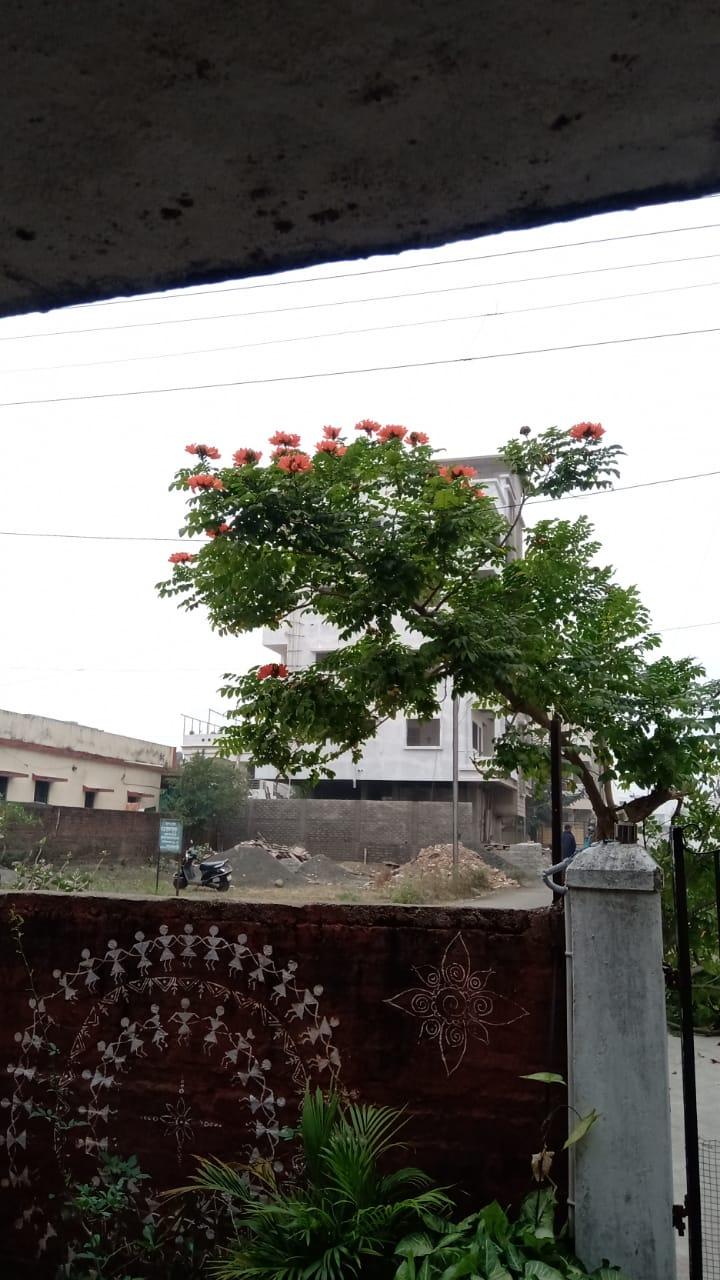
\includegraphics[scale=0.3]{home.jpeg}
	  \caption{Home, Nagpur}
	  \label{fig:Home}
	\vspace{2cm}
	\end{figure}
\begin{figure}

  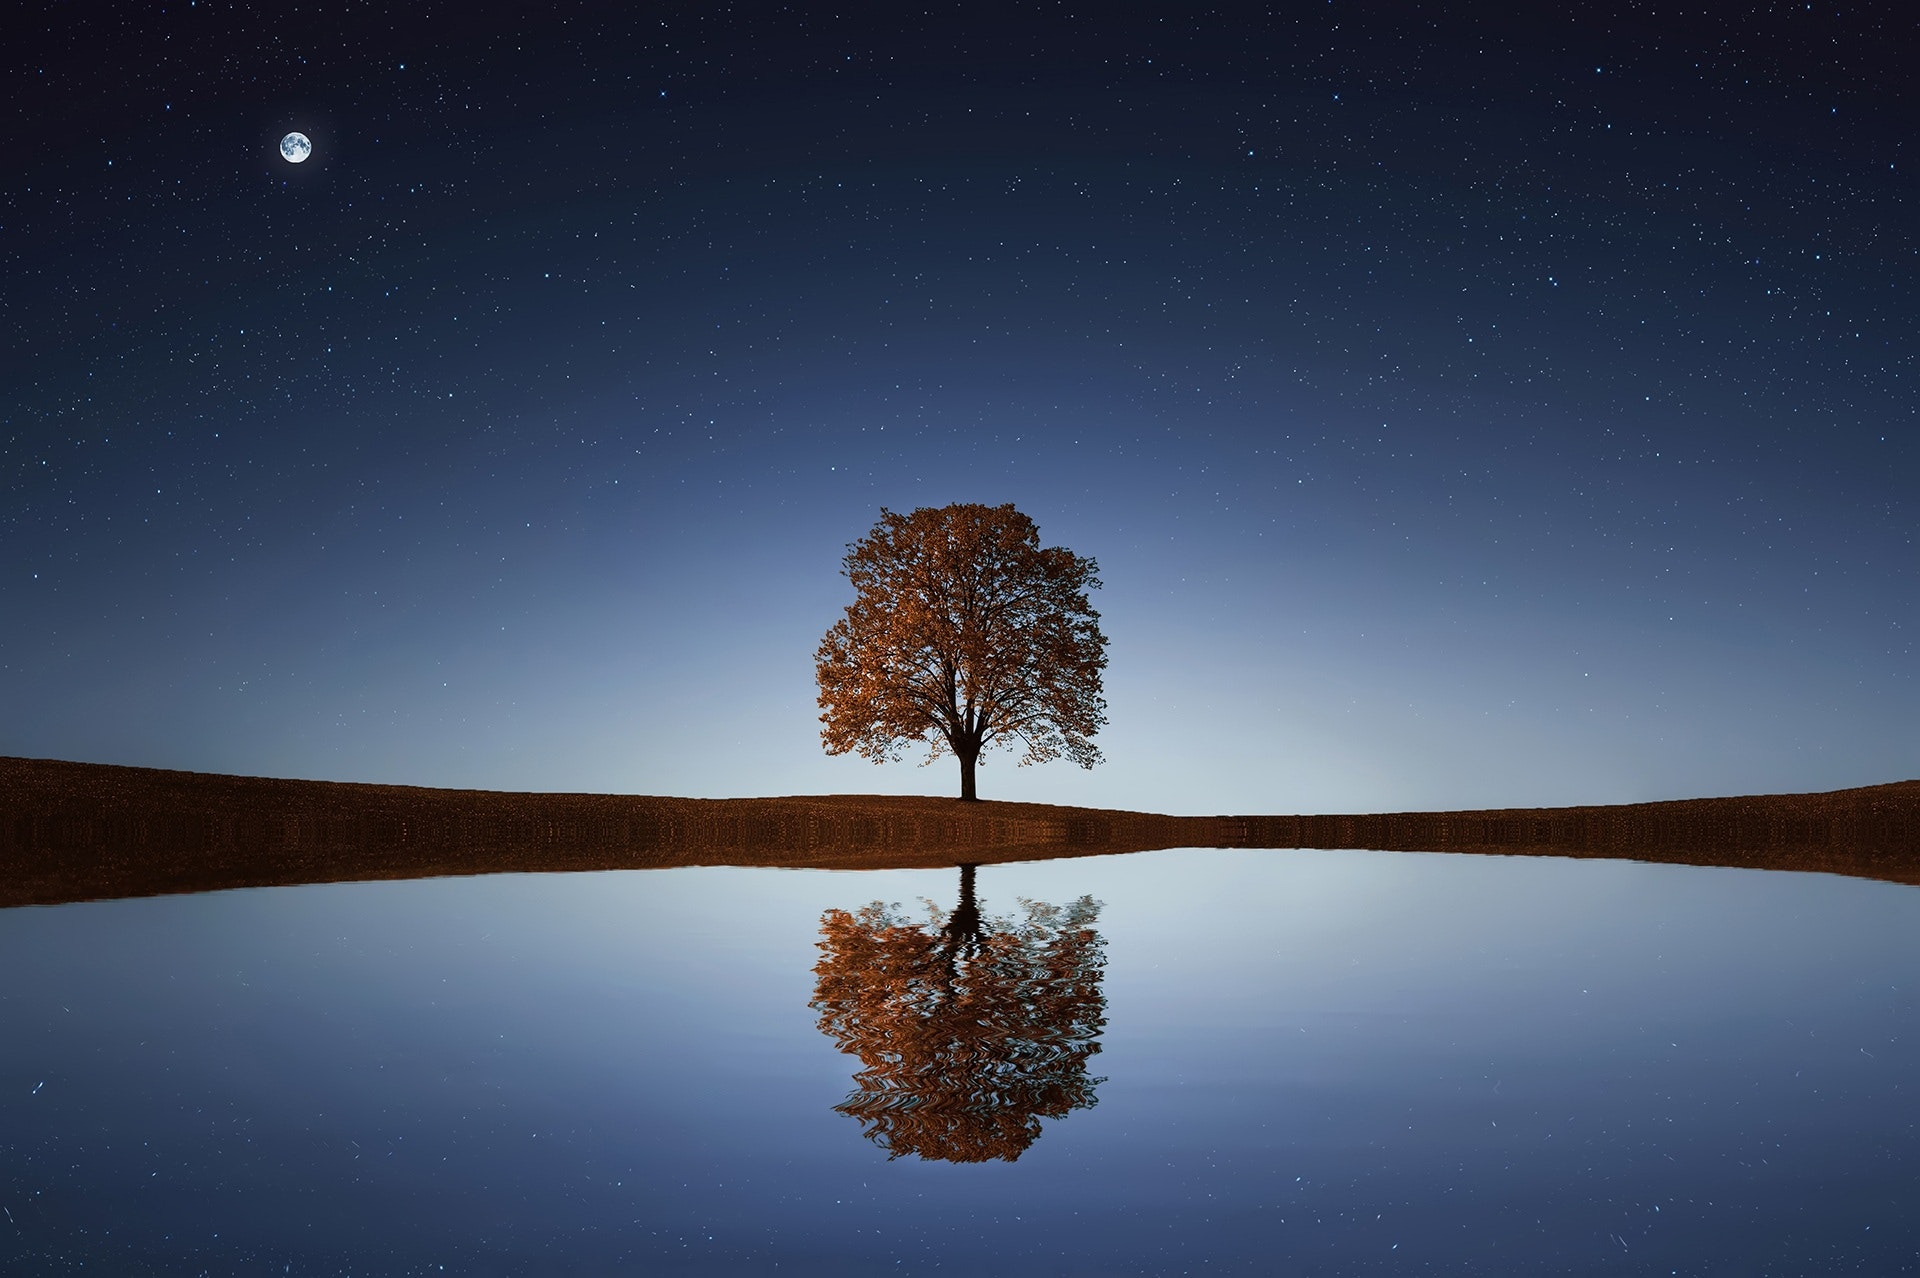
\includegraphics[width=\linewidth]{scenary1.jpg}
  \caption{A crystal clear waterbody}
  \label{fig:Scenary}
\end{figure}

\pagebreak 

\section{Tables}
\begin{table}[h!]
\begin{center}
\caption{Anime}
\label{tab:Table1}
\vspace{10mm}
\begin{tabular}{|l|c|c|}
\hline
\textbf{Anime} &\textbf{Protagonist} &\textbf{Antagonist}\\
\hline
One Piece & Monkey D. Luffy & Kaido\\
Naruto & Uzumaki Naruto& Uchiha Madara\\
Chainsaw Man & Deji & Gun Devil\\
\hline
\end{tabular}
\end{center}
\end{table}
\vspace{40mm}

\begin{table}[!ht]
\begin{center}
\caption{Sitcoms}
\label{tab:Table2}
\vspace{10mm}
\begin{tabular}{|l|c|c|}
\hline
\textbf{Subjects} &\textbf{Credits} &\textbf{Rating out of 10}\\
\hline
Linear Algebra and Univariate Calculus & 5 & 8\\
\hline
Foundations of Physics & 3 & 9\\
\hline
Datastructures and Algorithms 1 & 3 & 10\\
\hline
Digital Logic Design & 3 & 9\\
\hline
Descrete structures and Graph Theory & 3 & 8\\
\hline
\end{tabular}
\end{center}
\end{table}

\section{Include table from CSV}
\begin{tabular}{|c|c|c|}%
\hline1
\bfseries Name & \bfseries Age & \bfseries College
\csvreader[head to column names]{People.csv}{}
 {\\\hline\csvcoli&\csvcolii&\csvcoliii}\\
 \hline
 \end{tabular}




\end{document}